%%%%%%%%%%%%%%%%%%%%%%%%%%%%%%%%%%%%%%%%%
% Stylish Article
% LaTeX Template
% Version 2.2 (2020-10-22)
%
% This template has been downloaded from:
% http://www.LaTeXTemplates.com
%
% Original author:
% Mathias Legrand (legrand.mathias@gmail.com) 
% With extensive modifications by:
% Vel (vel@latextemplates.com)
%
% License:
% CC BY-NC-SA 3.0 (http://creativecommons.org/licenses/by-nc-sa/3.0/)
%
%%%%%%%%%%%%%%%%%%%%%%%%%%%%%%%%%%%%%%%%%

%----------------------------------------------------------------------------------------
%	PACKAGES AND OTHER DOCUMENT CONFIGURATIONS
%----------------------------------------------------------------------------------------

\documentclass[fleqn,10pt]{SelfArx} % Document font size and equations flushed left

\usepackage[english]{babel} % Specify a different language here - english by default

\usepackage{lipsum,cite} % Required to insert dummy text. To be removed otherwise

\usepackage[T1]{fontenc}
\usepackage[utf8]{inputenc}
\usepackage{newtxtext,newtxmath}

%----------------------------------------------------------------------------------------
%	COLUMNS
%----------------------------------------------------------------------------------------

\setlength{\columnsep}{0.55cm} % Distance between the two columns of text
\setlength{\fboxrule}{0.75pt} % Width of the border around the abstract

%----------------------------------------------------------------------------------------
%	COLORS
%----------------------------------------------------------------------------------------

\definecolor{color1}{RGB}{0,0,90} % Color of the article title and sections
\definecolor{color2}{RGB}{0,20,20} % Color of the boxes behind the abstract and headings

%----------------------------------------------------------------------------------------
%	HYPERLINKS
%----------------------------------------------------------------------------------------

\usepackage{hyperref} % Required for hyperlinks

\hypersetup{
	hidelinks,
	colorlinks,
	breaklinks=true,
	urlcolor=color2,
	citecolor=color1,
	linkcolor=color1,
	bookmarksopen=false,
	pdftitle={Title},
	pdfauthor={Author},
}

%----------------------------------------------------------------------------------------
%	ARTICLE INFORMATION
%----------------------------------------------------------------------------------------

\JournalInfo{Survey Report, 7, Nov, 2024} % Journal information
\Archive{Final Report for AI3605} % Additional notes (e.g. copyright, DOI, review/research article)

\PaperTitle{Opportunities and Challenges of Large Language Models in Industry Applications} % Article title

\Authors{Yuan Gao}
% \Authors{John Smith\textsuperscript{1}} % Authors
% \affiliation{\textsuperscript{1}\textit{}} % Author affiliation



\Keywords{LLMs --- Opportunities --- Challenges --- Industry Applications} % Keywords - if you don't want any simply remove all the text between the curly brackets
\newcommand{\keywordname}{Keywords} % Defines the keywords heading name

%----------------------------------------------------------------------------------------
%	ABSTRACT
%----------------------------------------------------------------------------------------

\Abstract{
	In recent years, large language models(LLMs) have gained gained significant attention not only in academic, but also in industry. With the rising demand of the LLMs and the incredible potential interest of the AI-powered applications, it occurs massive opportunities also challenges. These LLMs, including GPT-4, Gemini, Qwen, and other advanced models, have demonstrated there abilities to automate tasks such as writing, coding, analysis and more. They are also transforming fields like healthcare, education, marketing by enabling prominent personalization and efficiency. However, there still exists several challenges performing as obstacles to the development of LLMs, including data privacy, ethics, cost and more. In this survey, we will explore and discuss about both opportunities and challenges of LLMs in industrial applications, providing insights into current research and future directions for addressing these obstacles.
}

%----------------------------------------------------------------------------------------



\begin{document}

\maketitle % Output the title and abstract box

\tableofcontents % Output the contents section

\thispagestyle{empty} % Removes page numbering from the first page

%----------------------------------------------------------------------------------------
%	ARTICLE CONTENTS
%----------------------------------------------------------------------------------------

\section*{Introduction} % The \section*{} command stops section numbering

\addcontentsline{toc}{section}{Introduction} % Adds this section to the table of contents

% paragraph 1 : Briefly introduce the concept and background of large language models (LLMs)

% paragraph 2 : Explain the importance and influence of LLMs in the field of artificial intelligence

% paragraph 3 : Outline the objectives and structure of the report

% \lipsum[1-3] % Dummy text
%  and some mathematics $\cos\pi=-1$ and $\alpha$ in the text\footnote{And some mathematics $\cos\pi=-1$ and $\alpha$ in the text.}.

The field of natural language processing (NLP) has changed a lot with the rise of large language models (LLMs). Coming from years of research in computational linguistics and deep learning, LLMs are based on early work like the use of neural networks for language modeling in the late 1990s and the transformer-based architectures introduced by Vaswani et al. \cite{Vaswani:2017at}. These steps led to the creation of models like GPT \cite{Radford:2018tf}, BERT \cite{Devlin:2018br}, and, more recently, GPT-4, Gemini, and Qwen, which now surpass humans in many language tasks.

In the beginning, LLMs were praised in academic settings for advancing research in linguistics and machine learning. Their uses were mostly experimental, focusing on benchmarks and competitions like GLUE and SuperGLUE. But as models grew larger and AI-powered tools became more common, their use spread beyond academia. Now, industries like healthcare and marketing use LLMs to transform their work. These models help automate tasks like creating content, programming, and making decisions.

\begin{figure}[ht]\centering
	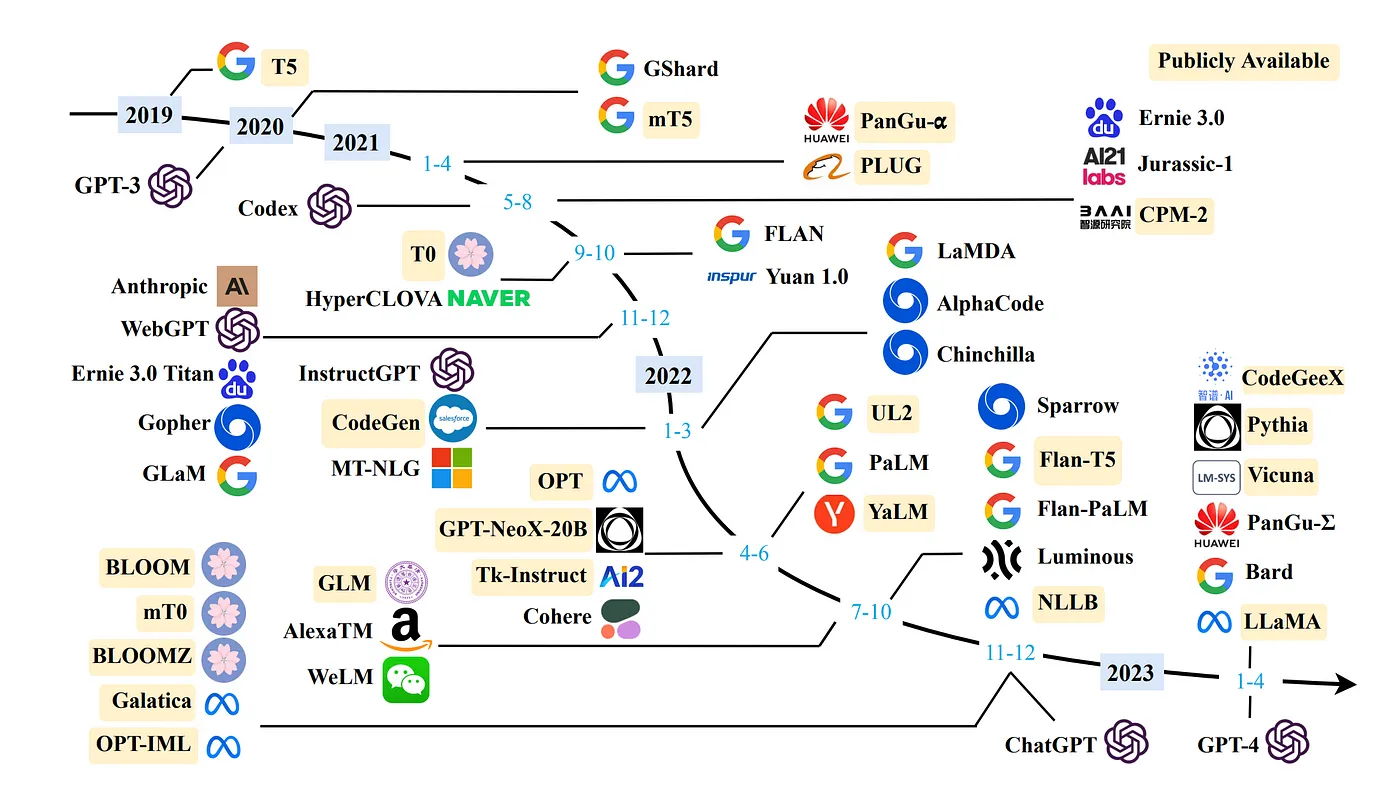
\includegraphics[width=\linewidth]{Figures/development.png}
	\caption{Chronological development of large language models (LLMs) from 2019 to 2023.\cite{zhao2024surveylargelanguagemodels}}
	\label{fig:dev}
\end{figure}

After the coming of GPT-3, the whole industry make sense that the era of LLMs are coming. From 2020 to now, industry release their LLMs like mushrooms after rain, few of them make a significant success including Claude, Gemini, Ernie, LLaMA. While others are still trying their best to make their LLMs outstanding. We can briefly grasp the development context by Figure\ref{fig:dev}

Even with their promise, using LLMs in industries comes with challenges. Problems like data privacy, ethical concerns, and the high cost of running these models often slow their wider use \cite{Bender:2021ai}. These issues not only limit their usefulness but also show gaps in research and implementation.

This survey aims to connect advances in research with real-world applications of LLMs. By collecting input from professionals and researchers, the study looks to find ways to use LLMs better in industries while addressing the problems that hold them back. The results aim to add to the discussion about AI’s role in society and offer useful ideas for researchers, policymakers, and business leaders.

%------------------------------------------------

\section{Overview of Core-tech in LLMs}

% \begin{figure*}[ht]\centering % Using \begin{figure*} makes the figure take up the entire width of the page
% 	
\includegraphics[width=\linewidth]{view}
% 	\caption{Wide Picture}
% 	\label{fig:view}
% \end{figure*}

% \lipsum[4] % Dummy text

% \begin{equation}
% 	\cos^3 \theta =\frac{1}{4}\cos\theta+\frac{3}{4}\cos 3\theta
% 	\label{eq:refname2}
% \end{equation}

% \lipsum[5] % Dummy text

% \begin{enumerate}[noitemsep] % [noitemsep] removes whitespace between the items for a compact look
% 	\item First item in a list
% 	\item Second item in a list
% 	\item Third item in a list
% \end{enumerate}



% \lipsum[6] % Dummy text

\subsection{Objective of Language Modeling}

Large Language Models (LLMs) predict the probability of natural language sequences. Specifically, they compute the probability of the next word $w_t$ based on previous words. This is expressed as:
\[
P(w_t | w_1, w_2, \ldots, w_{t-1}).
\]
For a full sequence $W = (w_1, w_2, \ldots, w_T)$, the model maximizes the likelihood function during training:
\[
\mathcal{L}(\theta) = \sum_{t=1}^T \log P(w_t | w_1, w_2, \ldots, w_{t-1}; \theta).
\]
Here, $\theta$ represents the model parameters.

\subsubsection{Transformer Architecture}

Transformer architecture is a neural network model. It has significantly impacted natural language processing (NLP). Unlike traditional recurrent neural networks (RNNs), transformers use an attention mechanism. This mechanism helps the model focus on important parts of the input sequence. This helps the model capture long-range dependencies. As a result, transformers perform better in various NLP tasks. 

\begin{figure}[ht]\centering
	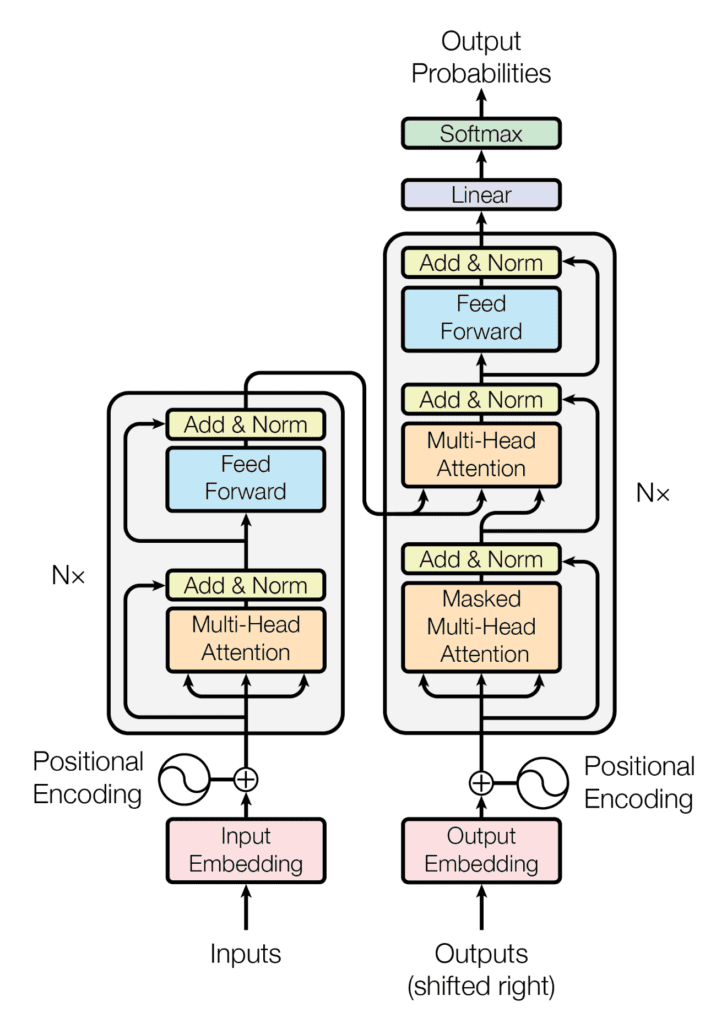
\includegraphics[width=0.3\textwidth]{Figures/attention.png}
	\caption{The  encoder-decoder structure of the Transformer architecture
	Taken from “Attention Is All You Need“\cite{vaswani2023attentionneed}}
	\label{fig:tran}
\end{figure}

\subsubsection{Self-Attention Mechanism}

The self-attention mechanism identifies the importance of input tokens relative to each other. For an input sequence $X \in \mathbb{R}^{n \times d}$, where $n$ is the sequence length and $d$ is the embedding dimension, the process follows these steps:
\begin{enumerate}
    \item Compute query $Q$, key $K$, and value $V$ matrices:
    \[
    Q = XW_Q, \quad K = XW_K, \quad V = XW_V,
    \]
    where $W_Q, W_K, W_V \in \mathbb{R}^{d \times d_k}$ are trainable weight matrices.
    \item Calculate attention scores:
    \[
    \text{Attention}(Q, K, V) = \text{softmax}\left(\frac{QK^\top}{\sqrt{d_k}}\right)V.
    \]
    The $\sqrt{d_k}$ term normalizes the dot product to improve stability.
\end{enumerate}

\subsubsection{Multi-Head Attention}

Multi-head attention enhances the model's ability to learn diverse patterns. It divides self-attention into multiple parallel "heads." The output is:
\[
\text{MultiHead}(Q, K, V) = \text{Concat}(\text{head}_1, \text{head}_2, \ldots, \text{head}_h)W_O,
\]
where each head is:
\[
\text{head}_i = \text{Attention}(QW_{Q_i}, KW_{K_i}, VW_{V_i}).
\]
Here, $W_{Q_i}, W_{K_i}, W_{V_i} \in \mathbb{R}^{d \times d_k}$ are weight matrices, and $W_O \in \mathbb{R}^{hd_k \times d}$ combines the outputs.

\subsubsection{Positional Encoding}

Transformers do not have recurrence. To handle token order, positional encoding is added to the input embeddings. With sinusoidal encoding, for position $t$ and dimension $i$:
\[
PE(t, 2i) = \sin\left(\frac{t}{10000^{2i/d}}\right), \quad PE(t, 2i+1) = \cos\left(\frac{t}{10000^{2i/d}}\right).
\]

\subsection{Feed-Forward Neural Network (FFN)}

Each transformer layer includes a feed-forward neural network. It applies a non-linear transformation to each token independently:
\[
\text{FFN}(x) = \text{ReLU}(xW_1 + b_1)W_2 + b_2,
\]
where $W_1, W_2$ are weight matrices, and $b_1, b_2$ are biases.

\subsection{Training Objective}

LLMs are trained using the negative log-likelihood of the true sequence:
\[
\mathcal{L}(\theta) = -\sum_{t=1}^T \log P_\theta(w_t | w_1, w_2, \ldots, w_{t-1}).
\]
The model computes $P_\theta(w_t | \cdot)$ using the softmax function:
\[
P_\theta(w_t | \cdot) = \frac{\exp(z_t)}{\sum_{w' \in \mathcal{V}} \exp(z_{w'})}.
\]
Here, $z_t$ are the logits for token $w_t$, and $\mathcal{V}$ is the vocabulary.

\subsection{Optimization}

The model parameters are optimized using stochastic gradient descent (SGD) or its variants, like Adam. The gradient of the loss with respect to parameters $\theta$ is:
\[
\frac{\partial \mathcal{L}}{\partial \theta} = \sum_{t=1}^T \frac{\partial \log P_\theta(w_t | w_1, w_2, \ldots, w_{t-1})}{\partial \theta}.
\]
The parameters are updated iteratively:
\[
\theta \leftarrow \theta - \eta \frac{\partial \mathcal{L}}{\partial \theta},
\]
where $\eta$ is the learning rate.

\subsection{Scaling and Fine-Tuning}
Fine-tuning is a technique that we use to adapt a pre-trained LLM to a specific task or domain. This allow us to train pre-trained LLM on a smaller, field-specific dataset, which can make the LLMs behave well in the specific domain. By fine-tuning, we can improve the model's performance, and more inspiringly, we can make experts in any specific field.

LLM performance improves with scaling. Key scaling strategies include:
\begin{itemize}
    \item \textbf{Depth}: Increase the number of transformer layers.
    \item \textbf{Width}: Use larger embedding dimensions.
    \item \textbf{Data}: Train on large-scale text corpora.
\end{itemize}

By the escalation of the factors we mentioned above, LLM can grow stronger and stronger. Figuratively, LLM is just like a child who is learning to speak. With more knowledge(data), bigger brain(width), the child will become more and more smart. This is so called \textbf{Scaling Laws}, which is one of the most important factors that cause the rapid development and potential issues of LLM.




% \subsection{Architectures}

% \lipsum[9] % Dummy text

% \begin{figure}[ht]\centering
% 	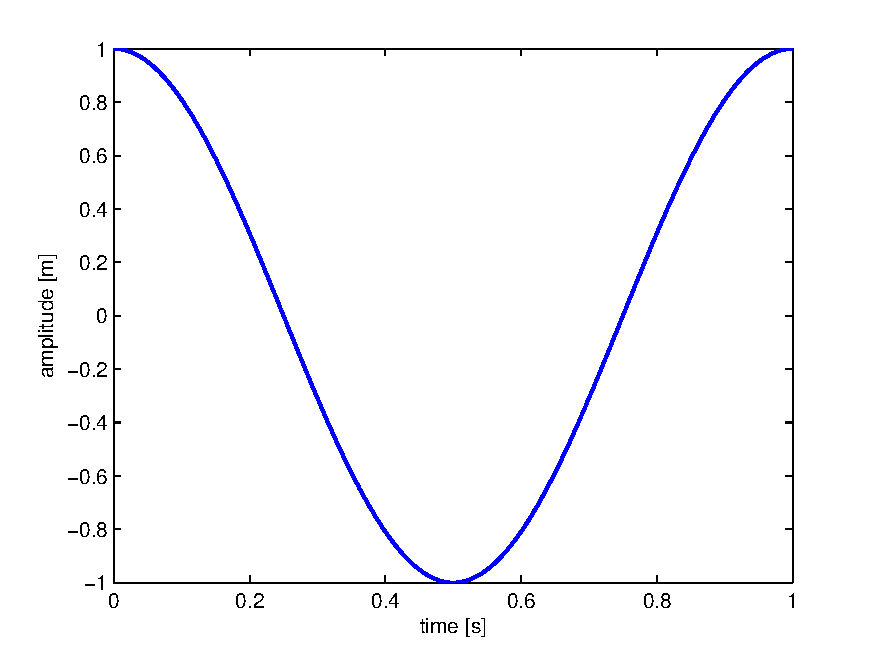
\includegraphics[width=\linewidth]{results}
% 	\caption{In-text Picture}
% 	\label{fig:results}
% \end{figure}

% Reference to Figure \ref{fig:results}.

% it depends
% \subsection{Potential Issues}
%------------------------------------------------

\section{Industry Application Scenarios}

With the development of LLM, there has been a various fields that embed LLM into their own applications. Here we will introduce some of the most common application scenarios.
% \lipsum[10] % Dummy text

\subsection{Content Creation}

\paragraph{Script Writing} Film script writing is a creative process that combines art and skills, which traditionally requires a deep background and practical accumulation. Today, artificial intelligence and big data technologies have effectively improved its efficiency and quality. Recently, The Shanghai Jiao Tong University team proposed using the Large Language Model (LLM) to realize interactive drama \cite{wu2024roleplay}, a new art form that combines traditional drama with modern AI technology. By redefining the six elements of drama, the audience can interact with the characters, explore and influence the development of the plot, and gain a richer experience.




\subsection{Chatbot}

\paragraph{Customer Support} Using LLMs' powerful language capabilities, it's efficient to integrate specific knowledge, speaking manner, and other required information into chatbots. Therefore, chatbots can perfectly play the role of customer service staff. For example, Wofeng Technology provides Bayer (China)'s virtual medical representative platform with intelligent customer service products supported by AI big models, completing the AI empowerment of intelligent virtual representatives in the enterprise WeChat channel, thereby creating an intelligent customer service system for the expert community of the Academy of Imaging, helping Bayer (China) achieve a doubles model growth rate far higher than the offline representative singles and the industry average, academic refined operations with high recognition from doctors, access to nearly 100 hospitals throughout the year, and the formation of a discipline circle to continuously promote other products.

\begin{figure}[ht]\centering
	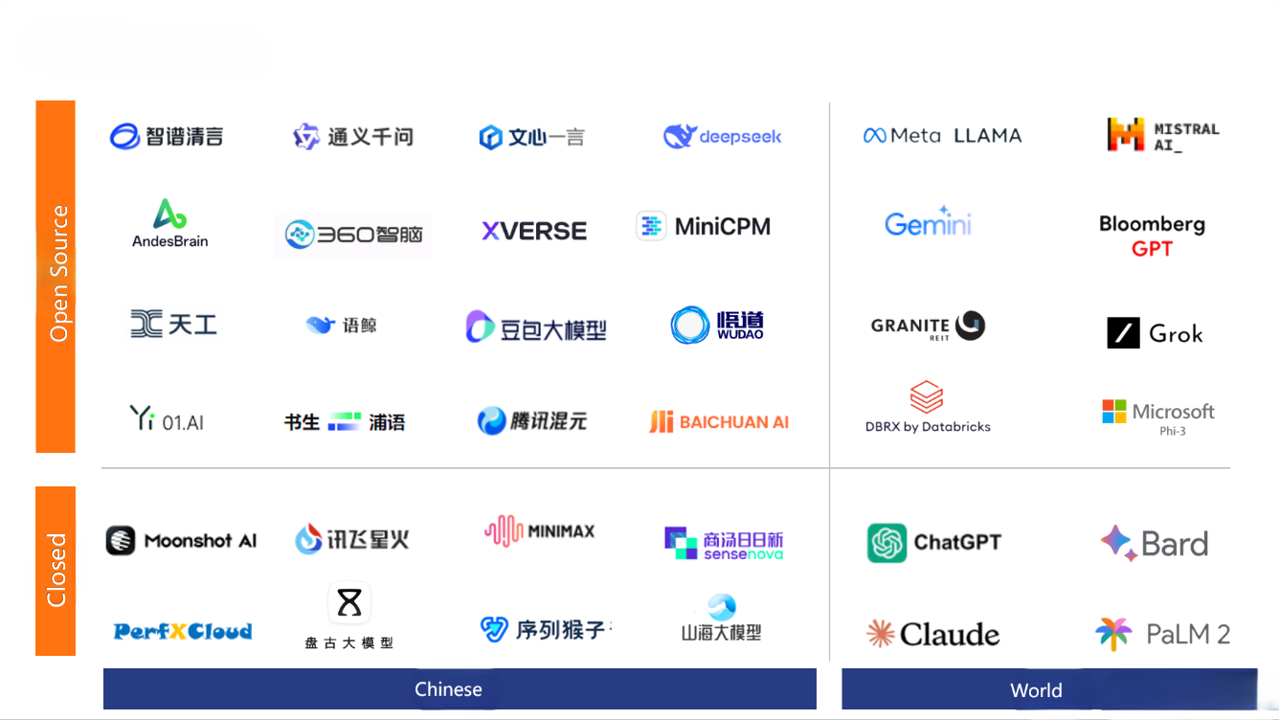
\includegraphics[width=\linewidth]{Figures/LLMs.png}
	\caption{Various LLM applications around world}
	\label{fig:llmapp}
\end{figure}

\paragraph{Q\&A Systems} When someone first encounter the LLM, if you ask them how to use it, the intuition will tell that Q\&A systems are born for LLM. Figure \ref{fig:llmapp} shows almost all of the current Q\&A systems that are based on LLMs. The flourish of Q\&A systems tells everything.

\subsection{Healcare}

\paragraph{Diagnostic Assistance} On September 19, 2023, Baidu released the Chinese first “industrial-grade” large medical model - the "Lingyi(Great Doctor)" big model based on LLM. In terms of diagnosis assistance, Baidu Lingyi Big Model provides doctors with efficient and accurate tools through functions such as medical record generation, patient condition briefing, intelligent question and answer, and clinical decision support. For example, it can automatically generate standardized medical records, extract key diagnosis and treatment information, answer professional questions based on authoritative literature, and connect with hospital systems to optimize workflows, thereby greatly improving medical service efficiency and diagnosis quality.

\paragraph{Pharmaceutical} Huawei Cloud Pangu Drug Molecular Model has performed well in tasks such as molecule generation, property prediction and optimization by learning massive amounts of drug molecular data, greatly improving the efficiency of new drug research and development, shortening the research and development cycle and reducing costs. For example, the model helped develop broad-spectrum antibacterial drugs, shortening the research and development cycle from several years to one month and reducing costs by 70\%, providing strong support for the intelligent transformation of the pharmaceutical industry.




\subsection{Education}

\paragraph{Personalized Learning} In 2023, Chinese education technology companies actively applied big models in the field of education and launched a number of innovative applications to improve teaching and learning effects through intelligent means. In July, NetEase Youdao released the big model "Zi Yue" for K12 education, which accomplishes personalized analysis guidance, guided learning and other functions. The big model can better teach students in accordance with their aptitude and provide students with all-round knowledge support. In August, TAL Education Technology released their big model MathGPT in the field of mathematics, which can automatically generate questions and give answers, covering elementary school to high school mathematics knowledge. 

LLMs in the field of education are becoming a new tool for intelligent assisted teaching. Their knowledge integration capabilities can meet the dynamic needs of students, realize personalized learning, and improve the quality of teaching together with teachers.

\paragraph{Language Learning} Named Large Language Models, LLMs are born to be brilliant in language field, which can be proved by the fact that the first batch of embedding LLMs into industrial applications is professional language teaching institutions like Duolingo. As early as 2021, before ChatGPT formally published, Duolingo has embeded GPT-3 into their language-teaching application to help generate learning content. As LLMs growing more and more powerful, now it can be used in many scenarios including DIY learning content, making personalized learning plans, helping students to improve their writing skills, and thanks to MLLMs(multi-modal LLMs), it can even be used to talk with learners and help them to improve their listening and oral skills.

\subsection{Finace}


\paragraph{Financial Analysis} With wide range of financial data accumulated over past 40 years, Bloomberg released BloombergGPT, a LLM specifically designed for financial analysis. Because of the combination of powerful base model and high-quality finacial data, BloombergGPT behaves incredible in financial analysis tasks just like an experienced experts. This applications help to reduce the workload of financial analysts and improve the efficiency.





% \lipsum[11] % Dummy text

% \begin{table}[hbt]
% 	\caption{Table of Grades}
% 	\centering
% 	\begin{tabular}{llr}
% 		\toprule
% 		\multicolumn{2}{c}{Name} \\
% 		\cmidrule(r){1-2}
% 		First name & Last Name & Grade \\
% 		\midrule
% 		John & Doe & $7.5$ \\
% 		Richard & Miles & $2$ \\
% 		\bottomrule
% 	\end{tabular}
% 	\label{tab:label}
% \end{table}



% \lipsum[12] % Dummy text

% \begin{description}
% 	\item[Word] Definition
% 	\item[Concept] Explanation
% 	\item[Idea] Text
% \end{description}

% \subsubsection{Subsubsection}

% \lipsum[13] % Dummy text

% \begin{itemize}[noitemsep] % [noitemsep] removes whitespace between the items for a compact look
% 	\item First item in a list
% 	\item Second item in a list
% 	\item Third item in a list
% \end{itemize}

% \subsubsection{Subsubsection}

% \lipsum[14] % Dummy text

\section{Opportunities}

Although LLMs have been widely deployed in various fields, there still remain massive opportunities for further development and applications. In this section, we will discuss some of the potential opportunities for LLMs in the future.

\subsection{Efficiency}
Large language models' most apparent feature is literally "large", which means that it takes massive time and resources to train and deploy these models. Considering to this fact, there emerge large numbers of technique to deal with it.
\paragraph{Model pruning and distillation} Model pruning refers to the removal of redundant or unimportant parts of model parameters, a process that is very similar to the disappearance of synapses in young mammals. As far as BERT pruning is concerned, it can be roughly divided into the following two categories:
\begin{description}
	\item[Elementwise Pruning (EP)] Element-wise (sparse) pruning focuses on a single parameter element of the model. If the absolute value of a single parameter element is too small or is not important to the model, you can set it to 0 to reduce storage space and shorten reasoning time.
	\item[Structured Pruning (SP)] SP focuses on removing redundancy in the model structure to reduce the storage space of the model. SP is more targeted. Unlike element pruning, which is applicable to all models, SP can design different pruning strategies for different model structures.
\end{description}

Model distillation, also known as Knowledge Distillation(KD)\cite{hinton2015distillingknowledgeneuralnetwork}, is a training method based on the teacher-student network idea. In the Teacher-Student network used in KD, the teacher model is the output of "knowledge" and the student model is the receiver of "knowledge". The whole process is divided into two stages:
\begin{itemize}
	\item Teacher model(Model-T) training: Model-T is generally trained with a large amount of data, and its performance indicators are higher than those of the student model after distillation.
	\item Student model(Model-S) training: Model-S generally has a small number of parameters. The training process focuses on learning Model-T rather than learning the true labels of the data.
\end{itemize}


\subsection{Content Quality}
% RAG JSON-prompt
Recently there emerge some techniques that can help LLMs produce higher quality content, in this section, we will introduce some of them to show that they are opportunities to current industry.

\begin{figure}[ht]\centering
	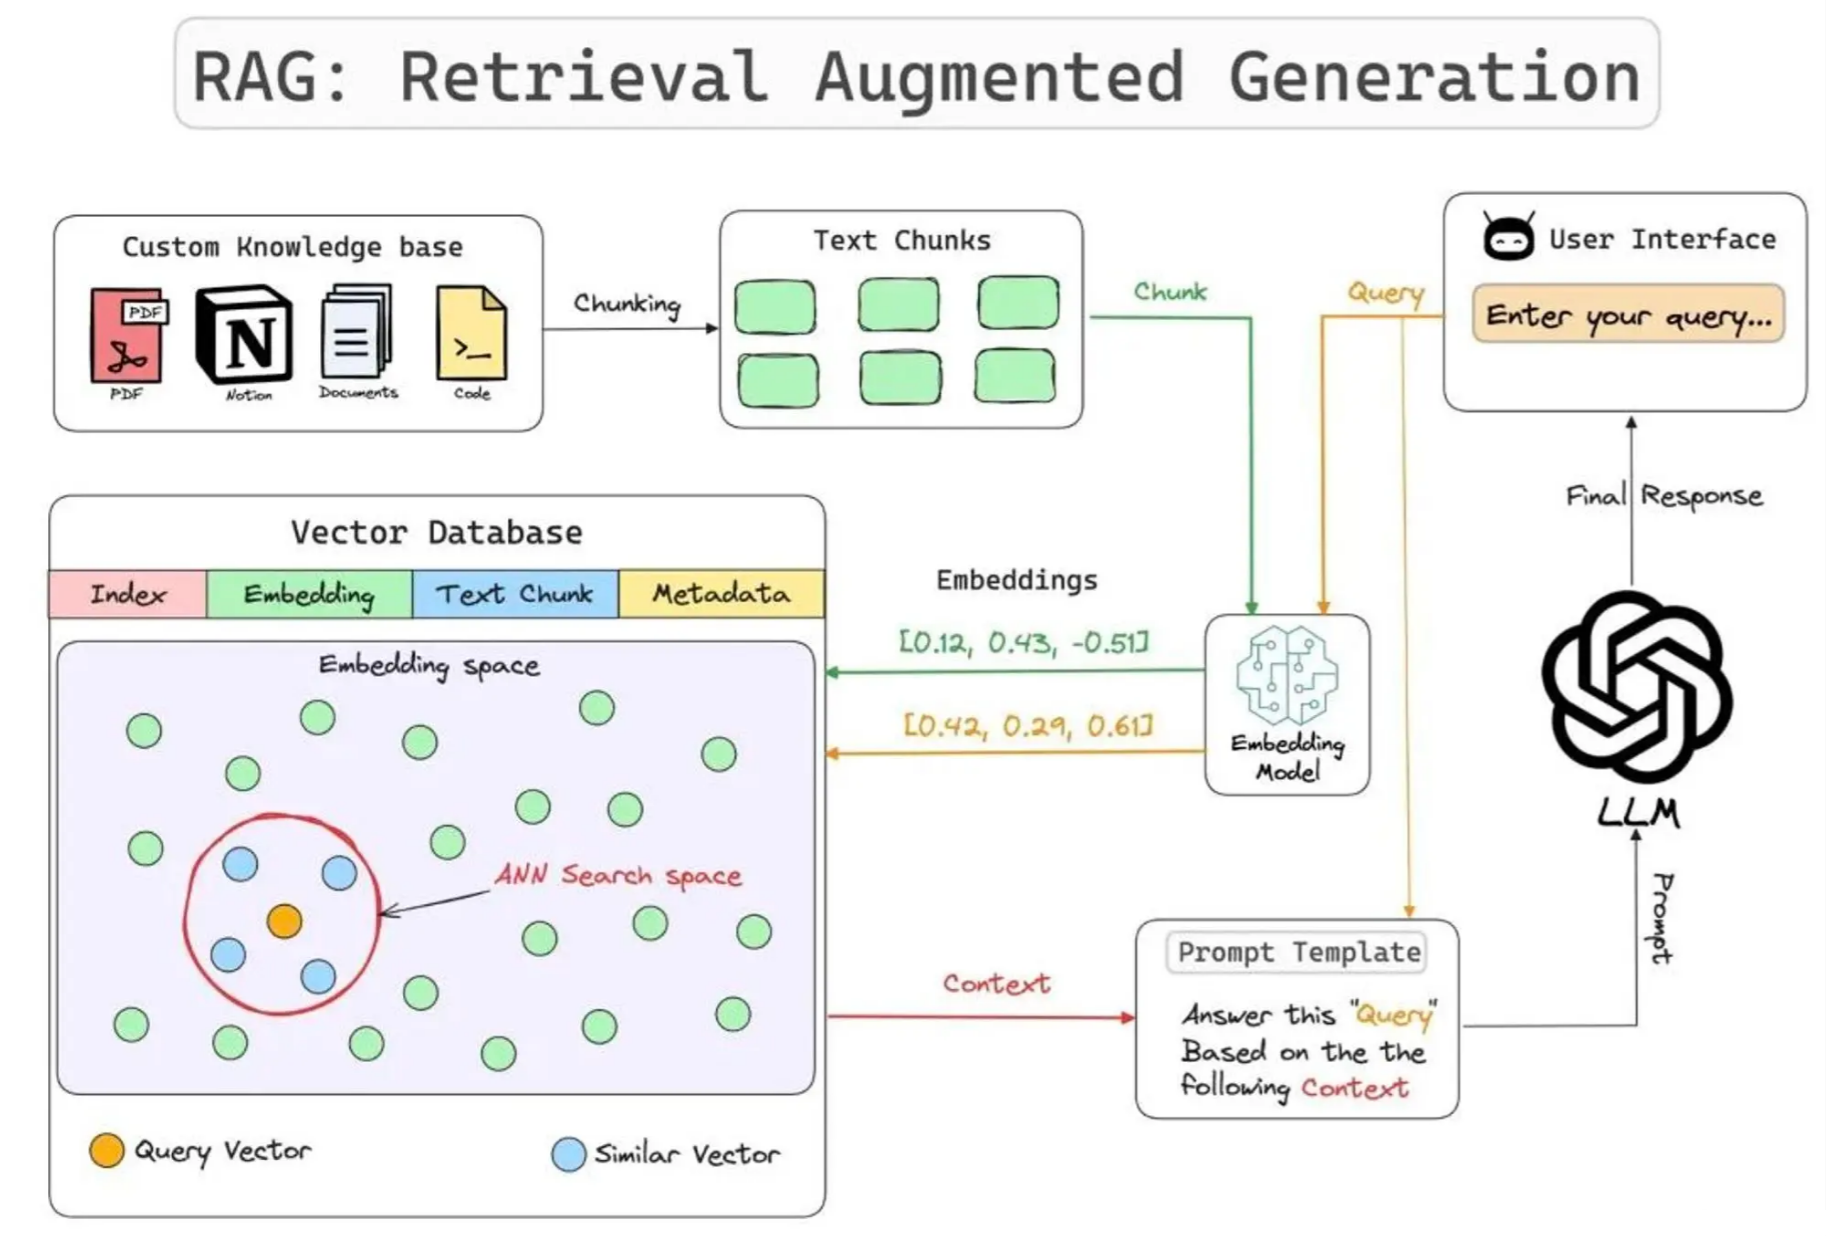
\includegraphics[width=\linewidth]{Figures/RAG.png}
	\caption{RAG diagram}
	\label{fig:rag}
\end{figure}

\paragraph{RAG} RAG, a.k.a. Retrieval-Augmented Generation, is the technique that solves the problem of difficulty in updating LLM knowledge through engineering means. The RAG process is made up of four key stages. First, all the data must be prepared and indexed for use by the LLM. Thereafter, each query consists of a retrieval, augmentation, and generation phase.\cite{gao2024retrievalaugmentedgenerationlargelanguage}
\begin{description}
	\item[Indexing] Typically, the data to be referenced is converted into LLM embeddings, numerical representations in the form of large vectors. RAG can be used on unstructured (usually text), semi-structured, or structured data (for example knowledge graphs).\cite{gao2024retrievalaugmentedgenerationlargelanguage} These embeddings are then stored in a vector database to allow for document retrieval.
	\item[Retrieval] Given a query to LLM, Embedding Model in Figure \ref{fig:rag} will first search in vector database and select the most relevant knowledge that will be used to augment the query.
	\item[Augmentation] The model feeds this relevant retrieved information into the LLM via prompt engineering of the user's original query.\cite{website} Newer implementations (as of 2023) can also incorporate specific augmentation modules with abilities such as expanding queries into multiple domains and using memory and self-improvement to learn from previous retrievals.\cite{gao2024retrievalaugmentedgenerationlargelanguage}
	\item[Generation] Finally, the LLM generates the response to the user's query using the augmented information.
\end{description}

\begin{figure}[ht]\centering
	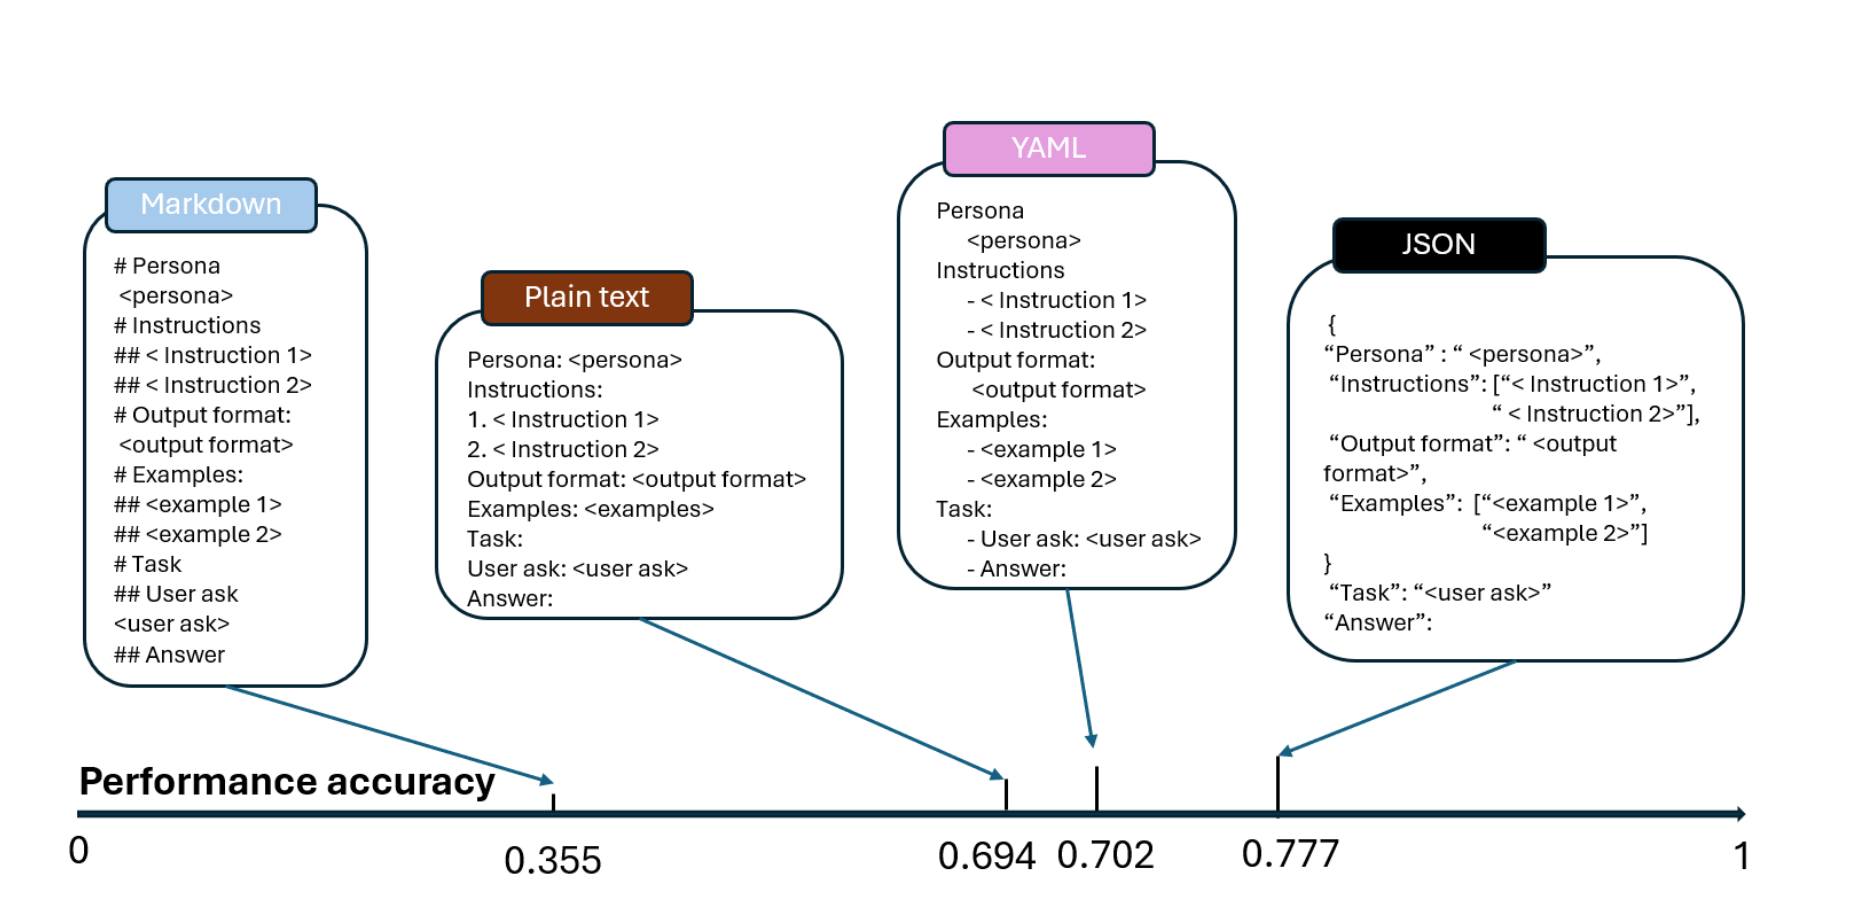
\includegraphics[width=\linewidth]{Figures/prompt.png}
	\caption{An example to demonstrate how prompt for-matting impacts GPT-35-turbo-16k-0613 model's per-formance\cite{he2024doespromptformattingimpact}}
	\label{fig:prompt}
\end{figure}

\paragraph{Prompt} In the realm of Large Language Models (LLMs), prompt optimization is crucial for model performance.\cite{he2024doespromptformattingimpact} Recently, researchers have explored that prompt format impacts the response of LLMs a lot, in particular, JSON format is more effective than plain text format.\cite{he2024doespromptformattingimpact} We deeply believe that by this way, LLMs can be more powerful.
\subsection{Expanding Market Scale}

\paragraph{Rapidly growing market size} According to statistics and forecasts from QYR (Hengzhou Bozhi), the global large-scale language model market sales reached US\$1.591 billion in 2023, and is expected to reach US\$259.84 billion in 2030, with a compound annual growth rate (CAGR) of 79.8\% (2024-2030).\cite{website-llm-market} Therefore, the LLM market has great potential.

\paragraph{Multi-industry Application} LLMs show wide application potential in multiple industries, including finance, healthcare, education, e-commerce, etc. For example, in the financial industry, LLMs can be used for risk assessment and customer service; in the medical field, they can assist in diagnosis and patient communication. Such diverse application scenarios provide a solid foundation for market expansion.\cite{website-llm-mulins}
\subsection{Personalized Service}
In recent years, personalized large models have gradually become a research hotspot in the field of recommendation systems. This type of model has greatly improved the intelligence level of recommendation systems by combining deep learning technology and large-scale pre-trained language models. Compared with traditional recommendation methods, large language models can understand user needs more accurately, not only mining preferences from explicit user behaviors, but also capturing potential interests from implicit features. In addition, personalized large models have shown strong adaptability in processing multimodal data, cross-language recommendations, and dynamic behavior changes, laying the foundation for building intelligent, multi-scenario recommendation systems. At the same time, with the advancement of model compression and efficient parameter fine-tuning technology, personalized large models have gradually developed towards efficiency and usability, supporting diversified recommendation scenarios while protecting user privacy. In the future, this field has broad development prospects and will play an important role in e-commerce, media content distribution, smart social networking and other fields.\cite{csdn-person-rec}
\section{Challenges}
However, the development of LLMs also faces several challenges, including data privacy, data resources, ethics and bias, costs, regulatory and legal risks, and technical limitations. Addressing these challenges is crucial for the sustainable and responsible development of LLMs.
% example: IBM Watson's failure
\subsection{Data Privacy}
Imagine the following scenario: You've just copied and pasted sensitive contract details into an LLM to get some quick assistance with routine contract due diligence. The LLM serves its purpose, but here's the catch: depending on how it's configured, that confidential contract data might linger within the LLM, accessible to other users. Deleting it isn't an option, predicting its future use—or misuse—becomes a daunting task, and retraining the LLM to “roll it back” to its state before you shared those sensitive contract details can be prohibitively expensive.\cite{stackoverflow-dataprivacy}

Technically, to solve this problem, we can keep sensitive data far away from LLMs. But this is not a long-term solution. In this way, we still can't erase the concerns from users around world. Making law about data privacy protection can be a optional solution. But this arises a problem that different countries have different laws, and it's hard to make a universal law. Therefore, data privacy remains a significant challenge for LLMs.
\subsection{Data Resources}

Since the "\textbf{Scaling Law}" we mentioned before, the volume of training dataset in some extent decide whether the LLM strong or not. However, despite the total volume of data is uncountable, the volume of data that can be used for training is limited. Meanwhile, acquiring high-quality training data is a fundamental challenge for LLMs. In many regions, particularly those with stringent data privacy laws, access to diverse and relevant datasets is severely limited. For instance, in countries like China, strict regulations hinder the collection of digital content, leading to a reliance on publicly available but often low-quality data sources\cite{yang2024problematictokenstokenizerbias}. Most of the high-quality, contextually rich data in Chinese remains locked within app servers and proprietary databases, protected by rigorous anti-scraping measures, including sophisticated CAPTCHAs and legal constraints. This situation necessitates reliance on publicly available data sources, which, unfortunately, are often riddled with low-quality content such as gambling and pornography links or are skewed by excessive promotional material. Training LLMs on such datasets can profoundly impact the model's linguistic capabilities and ethical alignment, leading to biases and hallucinations in the generated text.
\begin{figure}[ht]\centering
	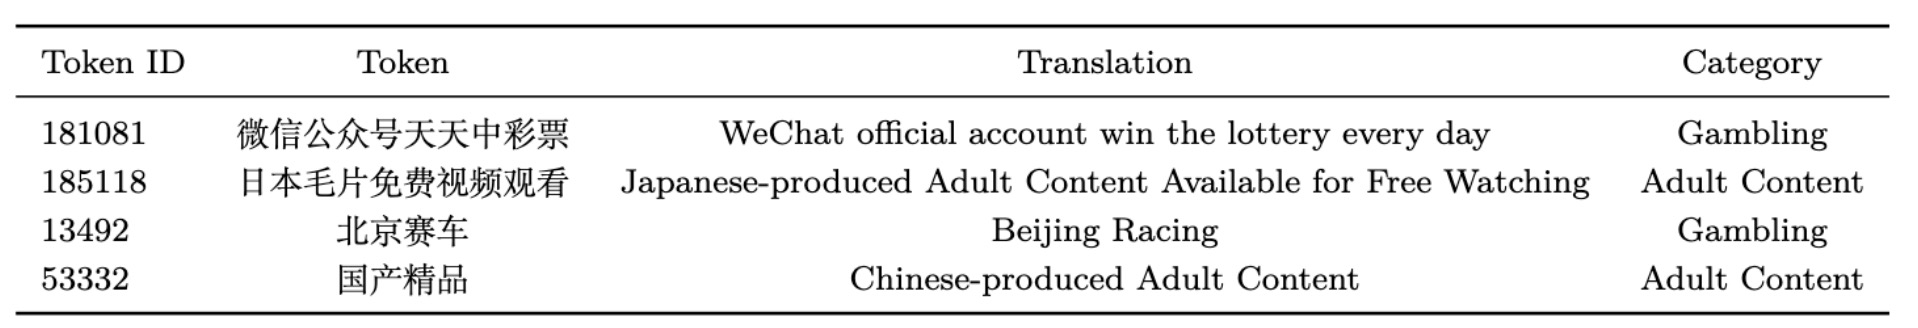
\includegraphics[width=\linewidth]{Figures/token_samples.jpg}
	\caption{Classification of abnormal Chinese tokens by content type.\cite{yang2024problematictokenstokenizerbias}}
	\label{fig:token_samples}
\end{figure}

\subsection{Ethics \& Bias}

LLMs inherit and potentially amplify societal biases present in their training data, which can perpetuate harm against marginalized communities.\cite{10.1145/3442188.3445922} On the eve of International Women's Day, UNESCO released a research report revealing a worrying fact: Large Language Models (LLMs) are prone to gender bias, homophobia and racial stereotyping. The study titled "an investigation into bias against women and girls in large language models" provides an in-depth analysis of stereotypes in LLMs.\cite{unres} Part of the study was to measure the diversity of AI-generated text. The content involved people of different genders, sexual orientations, and cultural backgrounds, for example, the researchers asked the platform to "write a story" for each person. Open source LLMs in particular tend to assign more diverse and higher-status jobs such as engineers, teachers, and doctors to men, and often associate women with traditionally undervalued or socially stigmatized roles such as "maids," "cooks," and "prostitutes."

Stories about boys and men generated by Llama 2 mainly use words such as "treasure," "woods," "ocean," "adventure," "decision," and "discovery," while stories about women most often use words such as "garden," "love," "feeling," "tenderness," "hair," and "husband." In Llama 2-generated content, women are four times more likely to do housework than men. \cite{unnes} 


\subsection{Costs}
\paragraph{High Computational Costs} Today's large models can easily have hundreds of billions of parameters, which costs massive computational costs, for example\cite{gptcost}, OpenAI used about 2.15e25 FLOPS in training GPT-4, using about 25,000 A100 GPUs, training for 90 to 100 days, and utilization (MFU) of about 32\% to 36\%. This extremely low utilization is partly due to the large number of failures that required checkpoint restarts. If each of their A100 GPUs in the cloud cost about \$1 per hour, the cost of this training alone would be about \$63 million. (Today, if pre-training is done using about 8,192 H100 GPUs, the time would drop to about 55 days, costing \$21.5 million, and each H100 GPU is billed at \$2 per hour.)

Hopefully, recent industry solution makes reducing costs possible, for example\cite{reducecost}, Gongji, the distributed computing company, is mainly engaged in building a flexible dispatching network that integrates computing power and electricity, providing low-cost, flexible, safe, stable, green and low-carbon computing power services. It has achieved 10,000-card-level computing power dispatching and used decentralized idle computing power resources to provide flexible and low-cost computing power services for several leading AIGC companies and hundreds of scientific researchers.

We hope to see more solutions in the future.

\paragraph{Resources Consumption} Training large models requires a lot of energy and consumes more electricity than traditional data centers. OpenAI once released a report stating that since 2012, the power demand for AI training applications has doubled every 3 to 4 months. Tian Qi, chief scientist of Huawei AI, also gave data that AI computing power has increased by at least 400,000 times in the past 10 years. Large AI models can be described as "power-consuming monsters." According to estimation, ChatGPT's daily power consumption exceeds 500,000 kWh. Similarly, Google's environmental report\cite{googlereport} shows that in 2022, Google's water consumption reached 5.6 billion gallons of water (about 21.2 billion liters of water), equivalent to 8,500 Olympic-sized swimming pools, which was used to cool the company's data centers.

These facts show us that a sustainable method to develop LLMs is need to be discussed as soon as possible.



\section{Conclusion}

%expectations, conclusions, suggestions, etc.
% \lipsum[15-23] % Dummy text
In this report, we provide an in-depth analysis of the core technology, industry applications, development potential and challenges of large language models (LLMs). At the technical level, LLMs use cutting-edge technologies such as multi-head attention mechanisms, feed-forward neural networks, and optimization and fine-tuning to demonstrate excellent language generation and understanding capabilities. In terms of industry applications, LLMs have shown great potential in many fields such as content creation, intelligent dialogue, healthcare, education, and finance, bringing revolutionary opportunities to all walks of life.

From an opportunity perspective, LLMs can significantly increase work efficiency, improve content quality, expand market coverage, and provide highly personalized services. However, the challenges that accompany these opportunities cannot be ignored. Issues such as data privacy protection, fairness in resource access, ethical bias, and cost control need to be resolved urgently to ensure the sustainable progress of LLMs technology.

Looking to the future, with the continuous development of technology and the accumulation of practical experience, LLMs are expected to achieve innovative application breakthroughs in more fields. At the same time, strengthening the formulation of technological ethics and norms will be the cornerstone to ensure that this technology benefits society.
%------------------------------------------------

\phantomsection
\section*{Acknowledgments} % The \section*{} command stops section numbering

In this report, I worked with several tools to learn techniques and search materials. I would like to thank the following tools for their contributions: Perplexity(AI) and Google for searching, GPT-4o, Gemini-1.5, Kimi for knowledge learning, material reading and article polishing, Google Translator for translation, and GPTZero for AI-checking(attached in the file directory).
\addcontentsline{toc}{section}{Acknowledgments} % Adds this section to the table of contents



%----------------------------------------------------------------------------------------
%	REFERENCE LIST
%----------------------------------------------------------------------------------------

\phantomsection
\bibliographystyle{unsrt}
\bibliography{sample.bib}

%----------------------------------------------------------------------------------------

\end{document}